\documentclass[12pt]{article}

% Language setting
% Replace `english' with e.g. `spanish' to change the document language
\usepackage[english]{babel}

% Set page size and margins
% Replace `letterpaper' with`a4paper' for UK/EU standard size
\usepackage[letterpaper,top=2cm,bottom=2cm,left=3cm,right=3cm,marginparwidth=1.75cm]{geometry}



% Useful packages
\usepackage{amsmath}
\usepackage{graphicx}
\usepackage{float}
\usepackage{indentfirst}
\usepackage{changepage}
\usepackage{bookmark}
\usepackage{listings}
\usepackage{xcolor}
\usepackage[most]{tcolorbox}

\definecolor{codeblue}{RGB}{0,0,180}
\definecolor{codegreen}{RGB}{0,120,0}
\definecolor{codegray}{RGB}{245,245,245}
\newtcolorbox{reportbox}[1]{
	colback=gray!15,
	colframe=blue!10!black,
	boxrule=1pt,
	arc=2mm,
	title=\textbf{#1},
	fonttitle=\bfseries\color{white},
	colbacktitle=blue!40!black
}


\let\oldtexttt\texttt
\renewcommand{\texttt}[1]{{\fontsize{11pt}{12pt}\selectfont\oldtexttt{#1}}}

\lstdefinestyle{verilogstyle}{
    basicstyle=\ttfamily\fontsize{10pt}{12pt}\selectfont,
    keywordstyle=\color{codeblue}\bfseries,
    commentstyle=\color{codegreen},
    numbers=left,
    numberstyle=\tiny\color{gray},
    stepnumber=1,
    numbersep=8pt,
    xleftmargin=3em,
    breaklines=true,
    tabsize=2,
    showstringspaces=false
}


\lstset{style=verilogstyle}

\setlength{\parindent}{0pt}
\begin{document}


\begin{titlepage}
	\centering

	\vspace*{5cm}

	{\Large ELEN20006\_ 2026\_ SM1 \par}
	{\Huge Digital System \par}
	{\Huge Digital Watch Project Report \par}
	\vspace{2cm}

	{\large Author \par}
	\large{\begin{tabular}{c l}
			1550486 & Selina Cheng \\
		\end{tabular}}
		
	\vspace*{10cm}


	{\large University of Melbourne \par}
	{\large \today \par}

\end{titlepage}

\pagenumbering{roman}
\tableofcontents
\setcounter{tocdepth}{2}
\newpage

\pagenumbering{arabic}


\section{Backup Strategy}
%=======================================================================
% 1
%=======================================================================
This project uses Git for data backup and version control. The forked repository is stored in the personal account on GitHub.
The committed code is pushed to the remote repository after each module is completed and tested. This ensures that the latest version of the code is always backed up and can be easily accessed from any location.

\section{Time Display}
	\subsection{Seven-segment Display Decoder for Dexadecimal Digits} %module 6.1 p.17

	\begin{figure}[H]
		\centering
		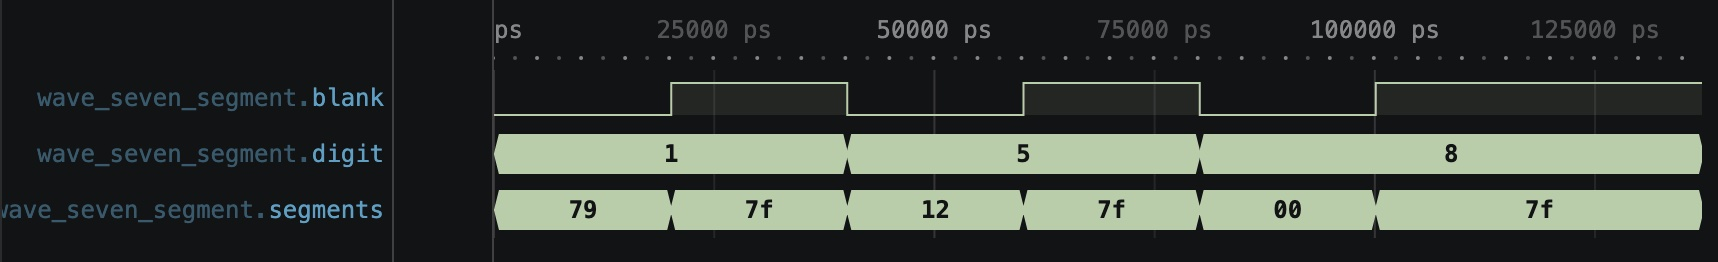
\includegraphics[width=0.9\linewidth]{figures/seven_segment.jpg}
		\caption{Waveform for \texttt{seven\_segment}.}
	\end{figure}

		Signal values are shown in hexadecimal.\\
		When \texttt{blank} is high, the output is 7f, which corresponds to 1111111 in binary — correct for an active-low display. The waveforms confirm the expected behaviour.
		\\
		\\

	\begin{reportbox}{Report 1}
	Explain why Verilator accepts \texttt{if (blank)} but not \texttt{if (ACTIVE\_LOW)}.
	\end{reportbox}

	\texttt{ACTIVE\_LOW} is a parameter, which will be known only at compile time and does not change during the runtime. Verilator will constant-fold \texttt{if (ACTIVE\_LOW)} in compilation.\\
	\\
	\texttt{if (blank)} is a conditional statement that depends on the value of \texttt{blank} at runtime, which can change during the execution of the program. So Verilator can treat it as a normal combinational logic.\\
	\\
	The reason Verilator may reject or warn about \texttt{if (ACTIVE\_LOW)} is usually because it expects a generate-time construct instead, or the branch becomes dead code, or the coding style implies hardware selection but the condition is constant.
	\subsection{Parametrised Up-Down Counter with Enable} %module 6.2 p.18

	\begin{figure}[H]
		\centering
		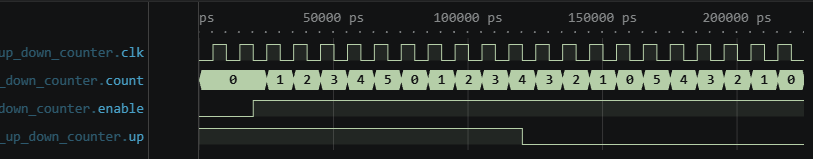
\includegraphics[width=0.9\linewidth]{figures/up_down_counter.png}
		\caption{Waveform for \texttt{up\_down\_counter}.}
	\end{figure}

		When enable is high, the counter starts to count.
		When \texttt{up} is high, the counter increments by one at every rising edge of the clock and goes down when \texttt{up} is low.\\
		The testbech sets \texttt{MAX} to 5, so the counter wraps around to 0 when it reaches 5 and wraps around to 5 when it goes down from 0.
		The waveforms confirm the expected behaviour.\\


	\begin{reportbox}{Report 4}
	Explain what binary-coded decimal (BCD) is. You may need to research it.
	\end{reportbox}

		Binary-coded decimal (BCD) is a way of representing decimal digits individually using binary. Each decimal digit is seperately represented by 4 bits in binary instead of showing full value in a long binary number.
	\subsection{Binary to Binary-Coded Decimal} %module 6.3 p.20 

	\begin{figure}[H]
		\centering
		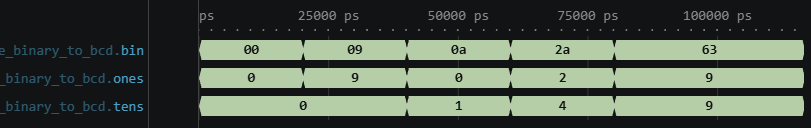
\includegraphics[width=0.9\linewidth]{figures/binary_to_bcd.png}
		\caption{Waveform for \texttt{binary\_to\_bcd}.}
	\end{figure}

		The binary inputs are shown in hexadecimal. The output values for \texttt{tens} and \texttt{ones} change to the corresponding digits of \texttt{bin} in BCD format immediately.\\
		\\
		For example, when \texttt{bin} is \texttt{0a}, which corresponds to 10 in decimal, \texttt{tens} changes to 1 and \texttt{ones} changes to 0 at the same instance.
	\subsection{Cascaded Hour-Minute-Second Counter with Enable} %module 6.4 p.20

	\begin{figure}[H]
		\centering
		\includegraphics[width=0.9\linewidth]{figures/hms_counter1.png}
		\includegraphics[width=0.9\linewidth]{figures/hms_counter2.png}
		\caption{Waveform for \texttt{hms\_counter}.}
	\end{figure}

		In the testbench setting for parameters, every day has 3 hours, each hour has 4 minutes and each minute has 5 seconds.\\
		\\
		When \texttt{enable} is high, the seconds counter starts to count. When \texttt{seconds} reaches 5, it wraps around to 0 and \texttt{minutes} increments by one. When \texttt{minutes} reaches 4, it wraps around to 0 and \texttt{hours} increments by one. When \texttt{hours} reaches 3, it wraps around back to 0.
	\subsection{Modulo N Counter} %module 6.5 p.22

	\begin{figure}[H]
		\centering
		\includegraphics[width=0.9\linewidth]{figures/mod_n_counter.png}
		\caption{Waveform for \texttt{mod\_n\_counter}.}
	\end{figure}

		When \texttt{enable} is high, the counter starts to count at every rising edge of the clock.
		The testbench sets N to 5, so the counter wraps around to 0 when it reaches 4. When both \texttt{rst} and \texttt{clk} are high, the counter is reset to 0.
	\subsection{Restartable Rate Generator} %module 6.6 p.23

	\begin{figure}[H]
		\centering
		\includegraphics[width=0.9\linewidth]{figures/restartable_rate_generator.png}
		\caption{Waveform for \texttt{restartable\_rate\_generator}.}
	\end{figure}

		Addition waveforms for \texttt{count} and \texttt{rst\_count} are shown for better understanding.\\
	\\
		When \texttt{enable} is high, the counter starts to count at every rising edge of the clock.
		The testbench sets \texttt{N} to 5, so the counter wraps around to 0 when it reaches 3. The \texttt{tick} is high when the counter reaches 3. When \texttt{tick} is high.\\
		\\
		The counter is reset to 0 at the next rising edge of the clock when both \texttt{rst} and \texttt{clk} are high, or when \texttt{tick} is high.\\
		\\

	\begin{reportbox}{Report 5}
	Explain how \texttt{localparam CounterWidth = \$clog2(CYCLE\_COUNT);} works.
	\end{reportbox}
		\texttt{\$clog2} calculates the ceiling of the logarithm base 2 of a given value. It returns the smallest integer that is greater than or equal to the logarithm base 2 of the input value.\\
		\\
		In this case, \texttt{CounterWidth} is the minimum number of bits required to represent the value of \texttt{CYCLE\_COUNT}.\\


	\begin{reportbox}{Report 6}
	In addition to running the provided testbench, write your own testbench verifying correct behaviour when \texttt{CYCLE\_COUNT = 1}.
	\end{reportbox}

		\texttt{ACTIVE\_LOW} is a parameter, which will be known only at compile time and does not change during the runtime. Verilator will constant-fold \texttt{if (ACTIVE\_LOW)} in compilation.\\
		\texttt{if (blank)} is a conditional statement that depends on the value of \texttt{blank} at runtime, which can change during the execution of the program. So Verilator can treat it as a normal combinational logic.\\
		\\
		The reason Verilator may reject or warn about \texttt{if (ACTIVE\_LOW)} is usually because it expects a generate-time construct instead, or the branch becomes dead code, or the coding style implies hardware selection but the condition is constant.


		\begin{lstlisting}[language=Verilog]
			`timescale 1ns / 1ps
			module wave_restartable_rate_generator_1cycle;
			reg  clk = 0;
			reg  run = 0;
			wire tick;

			restartable_rate_generator #(.CYCLE_COUNT(1)
			) dut (.clk (clk), .run (run), .tick(tick));

			always #5 clk = ~clk;

			initial begin
				$dumpfile("wave_restartable_rate_generator.vcd");
				$dumpvars(0, wave_restartable_rate_generator);

				#30;
				run = 1;
				#130;

				run = 0;
				#30;
				run = 1;
				#90;

				run = 0;
				#20 $finish;
			end
			endmodule
		\end{lstlisting}

		It generates waveform in figure 7. \texttt{tick} follows \texttt{run} at a new rising edge of \texttt{clk}.

	\begin{figure}[H]
		\centering
		\includegraphics[width=0.9\linewidth]{figures/restartable_rate_generator_1cycle.png}
		\caption{Waveform for testbench with \texttt{CYCLE\_COUNT = 1}.}
	\end{figure}
	\subsection{Variable-Speed Time Display} %module 6.7 p.25
		\begin{figure}[H]
			\centering
			\includegraphics[width=0.9\linewidth]{figures/top_time_display_v11.png}
			\includegraphics[width=0.9\linewidth]{figures/top_time_display_v12.png}
			\includegraphics[width=0.9\linewidth]{figures/top_time_display_v13.png}
			\caption{Waveform for \texttt{top\_time\_display\_v1}.}
		\end{figure}

			Signal of \texttt{SW} is shown in decimal. Signals of \texttt{HEX}s are shown in hexadecimal. Those values in binary are the corresponding \texttt{ACTIVE\_LOW} seven-segment display codes.\\
			\\
			For example, 40 represents binary \texttt{1000000}, corresponds to 0 on the display, 63 represents binary \texttt{1111001}, corresponds to 1 on the display, and 10 represents binary \texttt{0010000}, corresponds to 9 on the display.\\
			\\
			The time span for \texttt{SW = 2'b00} is not long enough to increment the \texttt{seconds} by 1Hz, so \texttt{seconds} remains at 0.
			When \texttt{SW = 2'b11}, \texttt{HEX}s increment in 50MHz, which is the same speed as \texttt{clk}.\\
			\\
			When \texttt{HEX0} reaches 10 (9 in terms of display), it wraps around to 40(0 in terms of display) and \texttt{HEX1} changes from 40 to 63.\\

\section{Settable Watch}
	%=======================================================================
	% 333333333333333333333333333333333333333333
	%=======================================================================
	\subsection{Fixed-frequency Fixed-duty PWM Generator} %module 7.1 p.28

	\begin{figure}[H]
		\centering
		\includegraphics[width=0.9\linewidth]{figures/pwm_generator.png}
		\caption{Waveform for \texttt{pwm\_generator}.}
	\end{figure}

		Testbench sets \texttt{pwm\_out} to be high for 8 cycles and low for
		2 cycles. The signal of \texttt{pwm\_out} confirms the expected behaviour, and resets the cycle when \texttt{rst} is high.

	\begin{reportbox}{Report 7}
	Explain why this module is called a PWM generator
	\end{reportbox}
		This module is called a PWM generator because it produces a Pulse Width Modulated (PWM) signal at \texttt{pwm\_out}. PWM signal is a repeating digital waveform which has period staying fixed and HIGH time corresponding to duty cycle. This module performs this behavior by implementing a modulor counter.\\


	\begin{reportbox}{Report 8}
	In mod\_n\_counter, rst takes priority over enable. Comment on the benefit of this
	design choice.
	\end{reportbox}
		This priority sequence insure that \texttt{rst} always immediately clean the old value regardless of the value of \texttt{enable}. If \texttt{enable} is given a higher priority, when \texttt{enable = 0}, \texttt{count} may stuck at oul value even though \texttt{rst} turns high.
	\subsection{Rising-edge Detector} %module 7.2 p.28

	\begin{figure}[H]
		\centering
		\includegraphics[width=0.9\linewidth]{figures/rising_edge_detector.png}
		\caption{Waveform for \texttt{rising\_edge\_detector}.}
	\end{figure}

		\texttt{rise} is up immediately after t\texttt{sig\_in} transition from low to high. When \texttt{sig\_in} remains high, \texttt{rise} goes back to low at the next rising edge of the clock.
	\subsection{Button Hold Detect} %module 7.3 p.28

	\begin{figure}[H]
		\centering
		\includegraphics[width=0.9\linewidth]{figures/button_hold_detect.png}
		\caption{Waveform for \texttt{button\_hold\_detect}.}
	\end{figure}

		Testbench sets \texttt{HOLD\_CYCLES} to be 3. In the generated graph, \texttt{held} is high for one cycle after \texttt{button} remains high for 3 cycle, and goes back to low if \texttt{button} remains high. So the waveforms confirm the expected behaviour.\\


	\begin{reportbox}{Report 9}
	Explain why the next-state logic may depend on the output held without violating
	the Moore FSM constraint.
	\end{reportbox}
		The calculation of \texttt{held} only depends on \texttt{count}, which is the current state. This does not violate Moore FSM as the output only depends on current state and input.  
	\subsection{Button Hold Pulse} %module 7.4 p.30

	\begin{figure}[H]
		\centering
		\includegraphics[width=0.9\linewidth]{figures/button_hold_pulse.png}
		\caption{Waveform for \texttt{button\_hold\_pulse}.}
	\end{figure}

		Testbench sets \texttt{HOLD\_CYCLES} to be 3. \texttt{held} is high for only one cycle after \texttt{button} remains high for 3 cycle, and goes back to low if \texttt{button} remains high.
		So the waveforms confirm the expected behaviour.\\


	\begin{reportbox}{Report 10}
	Explain what this module does. Justify your explanation by referring to the
	generated waveforms, being precise about timing.
	\end{reportbox}
		\texttt{pulse} rises high at the fifth complete cycle that a continuous high \texttt{button} encounter. It rises at the same time as the \texttt{clk} rises. \\


	\begin{reportbox}{Report 11}
	Explain how button\_hold\_pulse is a Moore FSM despite rising\_edge\_detector being
	Mealy.
	\end{reportbox}
		The FSM classification only applies to the FSM itself, not necessarily every submodule inside the overall design. The output is a direct combinatinal logic of the input. Using a Mealy input signal does not mean the output is Mealy too. 
	\subsection{Button Auto Repeat} %module 7.5 p.

	\begin{figure}[H]
		\centering
		\includegraphics[width=0.9\linewidth]{figures/button_auto_repeat.png}
		\caption{Waveform for \texttt{button\_auto\_repeat}.}
	\end{figure}

		Testbench sets \texttt{HOLD\_CYCLES = 8, REAPEAT\_CYCLES = 3}. When \texttt{button} is high, \texttt{pulse} goes high immediately until next cycle. At the 8th consecutive rising edges, \texttt{pulse} start to repeatly turning high for one cycle every three cycles.
	\subsection{Arming Latch} %module 7.6 p.32

	\begin{figure}[H]
		\centering
		\includegraphics[width=0.9\linewidth]{figures/arming_latch.png}
		\caption{Waveform for \texttt{arming\_latch}.}
	\end{figure}

		When {arm} is ever sampled high, \texttt{armed} begins to stay high continuously and backs to low when \texttt{disarm} is sampled high.  When \texttt{arm} and \texttt{disarm} are both sampled high, \texttt{armed} resets to zero because \texttt{disarm} takes higher priority..
	\subsection{Edit Mode Selector} %module 7.7 p.32

	\begin{figure}[H]
		\centering
		\includegraphics[width=0.9\linewidth]{figures/edit_mode_selector.png}
		\caption{Waveform for \texttt{edit\_mode\_selector}.}
	\end{figure}

		Testbench sets \texttt{HOLD\_CYCLES = 5}.\\
		A long press of button longer than 5 cycles turns the system into edit mode, where \texttt{mode\_enable} changes from 0 to 1. In edit mode for seconds and minutes, every press changes the system to the next mode, in sequence of seconds, minutes, to hours. When the system is in the hour editting mode, a press will end the edit mode.\\\\


	\begin{reportbox}{Report 12}
	Include your block diagram and explain the combinational logic you used for \texttt{enable\_counter}, \texttt{reset\_counter}, and \texttt{disarm}.
	\end{reportbox}

	\begin{figure}[H]
		\centering
		\includegraphics[width=0.9\linewidth]{figures/report_12.png}
		\caption{block diagram of \texttt{edit\_mode\_selector}.}
	\end{figure}
		

		The counter only advance when it is armed and a normal button press occurs. Therefore:
		\begin{lstlisting}[language=Verilog]
			assign enable_counter = armed && press;
		\end{lstlisting}
		This ensures enable is low whenever \texttt{armed} is low, only one increment occurs per press.
		\\
		The counter reset whenever edit mode is exited:
		\begin{lstlisting}[language=Verilog]
			assign reset_counter = disarm | !armed;
		\end{lstlisting}
		This immediately clears the mode counter back to zero after edit mode finishes.
		\\
		The system disarm when button is pressed while already on the last mode \texttt{(count == 2)}. Since the counter is modulo-3, valid modes are 0, 1, and 2. Therefore:
		\begin{lstlisting}[language=Verilog]
			assign disarm = armed && press && (count == 2);
		\end{lstlisting}
	\subsection{Editable Counter} %module 7.8 p.35

	\begin{figure}[H]
		\centering
		\includegraphics[width=0.9\linewidth]{figures/editable_counter.png}
		\caption{Waveform for \texttt{editable\_counter}.}
	\end{figure}

		Testbench sets {N = 3}. When \texttt{edit\_mode = 0}, counter advances by one at every tick and wraps around to 0 after reaching 3. Inside the edit mode, every cycle during \texttt{inc} is pressed increments \texttt{count} by one and \texttt{dec} does the opposite. When both \texttt{inc} and \texttt{dec} are pressed, they are ignored and the counter is unchanged.\\


	\begin{reportbox}{Report 13}
	Explain why \texttt{wire} was used instead of \texttt{logic} for the three event signals.
	\end{reportbox}
		These events are combinational logic only and do not store ports of submodule or any states. The valus are continuous assigned rather than variables that updated procedurally inside an \texttt{always\_comb} or \texttt{always\_ff} block. Therefore, using \texttt{wire} can show the intent clearly.
	\subsection{Key Synchroniser} %module 7.9 p.36

	\begin{figure}[H]
		\centering
		\includegraphics[width=0.9\linewidth]{figures/key_synchroniser.png}
		\caption{Waveform for \texttt{key\_synchroniser}.}
	\end{figure}

		The signal are in hexadeximal.\\ 
		This module use two stage flip-flop, so the corresponding update to the change of input always happens two cycle after. In the first two cycle, \texttt{key\_sync} is 0 because it is initialised to 0. It begins to be the bitwise invertion of input on the 3th cycles.\\ 
		\\
		For example, \texttt{4'hf} is 1111 in binary. The biwise invertion of it is a binary 0000 and a hexadecimal 0.
	\subsection{Decimal Display Driver} %module 7.10 p.36

	\begin{figure}[H]
		\centering
		\includegraphics[width=0.9\linewidth]{figures/decimal_display_driver.png}
		\caption{Waveform for \texttt{decimal\_display\_driver}.}
	\end{figure}

		The signals are shown in hexadecimal.\\
		The outputs of the displays are active-low 7-segment values, so the hexadecimal values correspond to the segment patterns. For example, \texttt{7'h40} corresponds to displaying digit 0 while \texttt{7'h79} corresponds to displaying digit 1.\\
		\\
		When \texttt{blank} becomes high, display output changes to \texttt{7'h7f}, which means all segments are OFF. For example, when \texttt{blank0} becomes 1 at around 100000 ps, \texttt{HEX0} changes from \texttt{7'h24} to \texttt{7'h7f}. Similarly, when \texttt{blank1} becomes 1, \texttt{HEX1} changes to \texttt{7'h7f}.\\
		\\
		The outputs update immediately after the corresponding input values and blanking signals change because the module is purely combinational logic and does not contain flip-flops.
	\subsection{Timekeeping (Watch V1)} %module 7.13 p.43

	\begin{figure}[H]
		\centering
		\includegraphics[width=0.9\linewidth]{figures/user_top_watch_v11.png}
		\includegraphics[width=0.9\linewidth]{figures/user_top_watch_v12.png}
		\includegraphics[width=0.9\linewidth]{figures/user_top_watch_v13.png}
		\includegraphics[width=0.9\linewidth]{figures/user_top_watch_v14.png}
		\caption{Waveform for \texttt{user\_top\_watch\_v1}.}
	\end{figure}
	% Waveform Explanation
		Testbench sets 10 cycles as one period of a second. The signals are shown in hexadecimal.\\
		\\
		Seconds counter starts to count at t = 0 and advances every 10 cycles. When \texttt{seconds\_disp} reaches 60, it wraps around to 0 and \texttt{minutes\_disp} increments by one. Testbench only runs for 2 minutes and 5 seconds, so \texttt{hours\_disp} remains 0.
		\\
		\\
	\begin{reportbox}{Report 14}
		Reflect on the role of the test suite.
	\end{reportbox}
	Testing cost grows exponatially as the combinations of possible input values grow. The test suite is important because manual testing on the FPGA board would be slow and unreliable. Even for basic timekeeping, it would need to wait long enough to check seconds rolling over to minutes, to hours, and hours wrapping back to zero. This take a long time for one version, and it would become impractical to repeat after every small change.\\
	\\
	As more features are added, such as edit mode, increment/decrement buttons, and different display states, the number of possible button combinations grows quickly. Testing all of these manually would be tedious and easy to do incompletely.\\
	\\
	Therefore, the automated test suite is valuable because it can repeatedly check expected behaviour much faster than manual testing. It also supports regression testing: when a new feature is added, the tests can immediately reveal whether an earlier function has been broken. This makes development safer, because old behaviour does not need to be manually rechecked from scratch every time.\\
	\\
	For example, testbenches can overide \texttt{CYCLES\_PER\_SECOND} to different values. If every second takes 50Ms, the testbench must has a significantly long simulating time length to cover every behaviors under testing. It is a good practice to allow parameters likes cycles count being changable, as simulation in smaller scale is easier for patterns tracking and debbugging.
	\subsection{Mode Selection (Watch V2)} %module 7.14 p.47

	\begin{figure}[H]
		\centering
		\includegraphics[width=0.9\linewidth]{figures/user_top_watch_v2.png}
		\caption{Waveform for \texttt{user\_top\_watch\_v2}.}
	\end{figure}
	% Waveform Explanation
	For every 50 cycles, \texttt{second\_disp} increments by one because this testbench overides \texttt{CYCLES\_PER\_SECOND} to 50.\\
	\\
	\texttt{blank} signals are off when \texttt{button[3]} is pressed. A continuous press logner than 50 cycles change the mode form normal to seconds edit mode. Every new individual long-press moves watch to next mode, following the order of: normal to seconds, seconds to minutes, minutes to hours, then hours to normal.\\
	\\
	After entering each edit mode, the corresponding blank signal repeatly stays low for 20 cycles then turns high for 5 cycles. Importing this signal to display modules as \texttt{blank} could achieves 2Hz 80\% duty cycle outputs.
	\subsection{Settable Watch (V3)} %module 7.15 p.47

	\begin{figure}[H]
		\centering
		\includegraphics[width=0.9\linewidth]{figures/user_top_watch_v31.png}
		\includegraphics[width=0.9\linewidth]{figures/user_top_watch_v32.png}
		\caption{Waveform for \texttt{user\_top\_watch\_v3}.}
	\end{figure}
	% Waveform Explanation
	This version adding edit funtion besides existing mode selection function. The testbench setting for \texttt{CYCLES\_PER\_SECOND} and the waveforms of \texttt{blank} signals are the same as in watch V2.\\
	\\
	During each edit mode, a short press of \texttt{button[2]} increments that part by one and repeatedly advances every 5 cycles if the press lasts longer than 25 cycles.  
	\subsection{Accurate Time Setting (V4)} %module 7.16

	\begin{figure}[H]
		\centering
		\includegraphics[width=0.9\linewidth]{figures/user_top_watch_v41.png}
		\caption{Waveform for \texttt{user\_top\_watch\_v4}.}
	\end{figure}

	\begin{figure}[H]
		\centering
		\includegraphics[width=0.9\linewidth]{figures/user_top_watch_v42.png}
		\caption{Waveform of transition form edit mode to minutes.}
	\end{figure}
	% Waveform Explanation
	Pressing \texttt{button[3]} in seconds edit mode changes the mode to minutes edit mode. As input of \texttt{button} changes to 8, \texttt{seconds\_edit} swiches low and \texttt{minutes\_edit} rises high at the next cycle.\\
	\\
	In module \texttt{restartable\_rate\_generator}:
	\begin{lstlisting}[language=Verilog]
		assign rst_count    = !run || tick;
	\end{lstlisting}
	\texttt{rst\_count} rises high when input \texttt{run = 0}. Therefore, reset of the cycles count for \texttt{seconds\_tick} could be correctly trigger by setting \texttt{run} low when the edit button is pressed during seconds editing mode.\\
	\\
	After the transition of edit mode from \texttt{seconds\_edit} to \texttt{minutes\_edit}, signal \texttt{count} inside rate generator resets to 0 then advances every new cycle. So the \texttt{seconds\_tick} does not rise high until reaching the 50th cycle.\\
	\\  
	\begin{reportbox}{Report 16}
		Does your design cause multiple resets? Why is this not a problem?
	\end{reportbox}
	\texttt{rst\_count} rises high when input \texttt{run = 0}. It generates high signal lasting few cycles following \texttt{run}. The counter stops at one when reset is high. This does not result in unexpected behaviour.
	\begin{reportbox}{Report 17}
		Reflect on your experience in previous lab classes.
	\end{reportbox}
	VS Code simulation enviroment can execute most of the developement procedures except baord compilation. Debbugging and code compilation usually take a long time on Quartus. VS Code enviroment integrates testbench, waveform, and fromal verification suit together improves efficiency by a lot.
	\begin{reportbox}{Report 18}
		Assume the 50 MHz clock on the DE1-SoC board is accurate to within 50 ppm. How many seconds might your watch drift over a 24-hour period?
	\end{reportbox}
	50ppm = 0.00005 = 0.005\% and 24 hours equals to 24×3600 = 86400 seconds. So the drift will be 86400 × 0.00005 = 4.32 seconds.


	\newpage

\section{Formal Verification}
	\begin{reportbox}{Report 1}
		When a module needs to be extended mid-design, several approaches are possible. Can you think of any other options? Justify your choices and discuss their trade-offs.
	\end{reportbox}
	Another option is to make the original module more general by adding parameters or optional ports, so that the old and new behaviours are selected by configuration rather than by maintaining two separate copies. In some cases the shared logic can also be factored into a smaller helper module, with two wrapper modules exposing the old and new interfaces.\\
	\\
	For this case, I would copy the original module, extend the copy, and rewrite the original as a thin wrapper around the extended version. I would keep the old module name for compatibility, for example \texttt{button\_auto\_repeat}, and name the new one according to the added behaviour, such as \texttt{button\_auto\_repeat\_no\_initial} or \texttt{button\_auto\_repeat\_extended}.\\
	\\
	This keeps existing code and tests working, because anything that instantiates the old module still sees the same interface and behaviour. At the same time, the new module can provide the extra functionality without duplicating most of the logic. The disadvantage is that there are now two module names to maintain, and the wrapper
	adds a small amount of indirection. However, this is usually better than modifying the original in place, which risks breaking earlier designs, or keeping two unrelated copies, which can diverge and become harder to debug.\\
	\begin{reportbox}{Report 2}
		Do the assertions above fully capture the behaviour of an up-down counter with reset? If not, identify any behaviours left unspecified, or any properties a reasonable person might expect that the assertions do not guarantee.
	\end{reportbox}
	The assertions do not fully specify all behaviour. For example, they do
	not check for unknown (\texttt{X}) values, combinational glitches between clock edges, or whether reset is synchronous or asynchronous. They verify the main functional behaviour, but not every possible implementation detail.\\
	\begin{reportbox}{Report 3}
		The configuration file verifies the counter for three specific values of MAX. Since this does not cover all possible values, how would you formally prove correctness when this module is used in a larger design?
	\end{reportbox}
	Testing only three values of \texttt{MAX} does not prove the module correct for all parameter choices. In a larger design, I would prove the counter after parameter specialisation: each instantiated counter has fixed values of \texttt{MAX} and \texttt{WIDTH}, so the formal tool only needs to prove correctness for those actual instances.\\
	\\
	I would also keep assertions inside or bound to the counter module, so every
	instance is checked with its own parameters. The proof should include assumptions that the parameters are valid, such as \texttt{MAX >= 0} and
	\texttt{(1 << WIDTH) > MAX}.\\
	\begin{reportbox}{Report 4}
		Include the counterexample waveform. The general reason for this failure was explained above; use the waveform to identify the specific counterexample the checker found and explain why it is one. Then explain why restoring the assertion allows the induction step to succeed.
	\end{reportbox}
	\begin{figure}[H]
		\centering
		\includegraphics[width=0.9\linewidth]{figures/report4.png}
		\caption{Waveform for the counterexample.}
	\end{figure}
	It starts at step 4 count = 0 and reversely decrements to 7 which is larger than MAX=4. This does not trigger the ignored assertion so basecase test is passed but induction is not.

\section{Stopwatch}
	\begin{reportbox}{Report 5}
		Before reading further, sketch how you would approach the design.
	\end{reportbox}
	I will amend module top\_time\_display\_v1 by adding additional button inputs for start/stop and reset time.\\
	\begin{reportbox}{Report 6}
		Using a feature layering approach, how would you decompose the stopwatch into layers? Describe the responsibility of each layer.
	\end{reportbox}
	There will be layers in the module. Timekeeping layer reponse to count time and react to start/stop and reset button. Display layer is responsible to transfer hms digits into HEX led display.
	\begin{reportbox}{Report 7}
		Draw a block diagram of the design described above, clearly showing the data path and control signals. Compare it with your initial sketch from Section 4.2 and comment on any differences.
	\end{reportbox}
	\begin{figure}[H]
		\centering
		\includegraphics[width=0.9\linewidth]{figures/report7.png}
		\caption{Block diagram for data path of stopwatch.}
	\end{figure}
	Latch function is added along with new module and new funtion for a button. \\
	\begin{reportbox}{Report 8}
		Explain how your implementation satisfies the first-tick timing constraint: the first centisecond increment must occur one centisecond after enable goes high, not sooner.
	\end{reportbox}
	When enable goes high, the counter does not increment immediately. The \texttt{restartable\_rate\_generator} first counts one centisecond worth of clock cycles. Only after this delay does it produce a one-cycle tick pulse. The cascade counter increments only when tick is high. Therefore, the first increment occurs exactly one centisecond after enable goes high, not sooner.\\
	\begin{reportbox}{Report 9}
		Draw a diagram showing how this is implemented in hardware.
	\end{reportbox}
	\begin{figure}[H]
		\centering
		\includegraphics[width=0.9\linewidth]{figures/report9.png}
		\caption{Assumption state diagram for \texttt{stopwatch\_control}.}
	\end{figure}
	\begin{reportbox}{Report 10}
		Draw the FSM state diagram before implementing it. After completing the implementation, note any differences between your diagram and the final design, and reflect on what caused them.
	\end{reportbox}
	Original initial state falsly combined two states: default state should not has rst high but make rst high as an independent state. Follows initial idea, clk should be consider as an input that effects state too because rst is a one cycle event then the state shift back.\\
	\\
	The final design followed hints to encode states by output:
	\begin{figure}[H]
		\centering
		\includegraphics[width=0.9\linewidth]{figures/report10.png}
		\caption{State diagram for final design for \texttt{stopwatch\_control}.}
	\end{figure}

\section{Timer}
	\begin{reportbox}{Report 11}
		Find the datasheet for the 74LS193 synchronous 4-bit up/down counter. Using the schematic diagram in the datasheet, explain how the borrow output is generated and why it behaves as it does.
	\end{reportbox}
	\begin{figure}[H]
		\centering
		\includegraphics[width=0.9\linewidth]{figures/74LS193.png}
		\caption{Schematic diagram of 74LS193.}
	\end{figure}
	Borrow is a output of a NAND gate taking inputs from: !down count, !$Q_d$, !$Q_c$, !$Q_b$, and !$Q_a$. So the borrow output goes low only when all these inputs are zero. That means the counter is currently at zero, and a down-count pulse is being applied. So the borrow output is active-low.\\
	\\
	So if several 74LS193 counters are connected together, the borrow output from the lower 4-bit counter can drive the down-count input of the next higher counter. When the low-order counter goes from 0000 to 1111, it produces a borrow pulse telling the next counter to decrement by one.
	\begin{reportbox}{Report 12}
		Describe your integration plan: which features did you implement first, and why?
	\end{reportbox}
	I first implement Mode selection function because it is small and similar to watch part while count down function can not independenty work. If count down module independently simulating, time will start at 0 and can not test count down function as timer can't change it's time to something larger than 0 so the editable countdown submodule is enabled.
	\begin{reportbox}{Report 13}
		The timer requires an FSM to manage its three modes. Explain your FSM design: what are the states, what are the transitions, and how did you encode the states? Justify your choices.
	\end{reportbox}
	\begin{figure}[H]
		\centering
		\includegraphics[width=1\linewidth]{figures/report13.png}
		\caption{State diagram of modes selection for \texttt{user\_top\_timer\_v1}.}
	\end{figure}
		\begin{lstlisting}[language=Verilog]
			logic [2:0] mode_enable;
			logic not_editting;
			logic time_not0;
			logic running = 1'b0;

			always_ff @(posedge clk) begin
				if (not_editting && ((time_not0 & start_stop)  // paulse or staet when time > 0
					|| (!time_not0 && running)))  //stop when reach 0
				running <= !running;
				if (!not_editting) running <= 1'b0;
			end

			assign not_editting = (mode_enable == '0);
			assign time_not0 = ({hours, minutes, seconds} != '0);

			edit_mode_selector #(
				.HOLD_CYCLES(CYCLES_PER_SECOND)
			) u_mode_selector (
				.clk(clk),
				.button(button[3] && !running),
				.mode_enable(mode_enable)
			);		

		\end{lstlisting}
	
\section{Timepiece}
	\begin{reportbox}{Report 14}
		Looking back across both assignments, reflect on your experience designing and implementing a digital watch on an FPGA. What went well, what was harder than expected, and what would you do differently if you were starting over?
	\end{reportbox}
	First of all, I will make sure I read through all the hints and restrictions as well as carefully checking my comprehension of the specification is well aligned. I redid my design so many times just because i did not read through whole instruction but start coding as soon as some ideas popped out. Checking specification through reading test codes and assertion files is a efficient way for me, a poor english user. \\
	\\
	I didn't know that internal signals are visible before the end of assignment 1. Debbuging with vaporview is fun and  way more efficient than silently looking at plain code.\\
	\\
	Integrating part is harder to debbug than thought.\\
	\begin{reportbox}{Report 15}
		Estimate how much time you saved compared to having used only Quartus. Breakdown the time savings between better editing features, linting, and automated tests plus formal verification. Without these tools, at what stage would you have discovered a problem, and how much harder would it have been to locate and fix the source of the error?
	\end{reportbox}
	More than ten if not hundred times of time would be lost at debbugging just in Quartus. I could only found a problem after countless slow compilation and implemented on the board than found out nothing would work.\\
	\\
	Automated tests and formal verification probably saved the most time. Without them, many bugs would only appear after FPGA testing, where you only see strange behaviour instead of the actual failing condition. Assertions and testbenches often located problems immediately.\\
	\\
	Linting also helped a lot by catching width mismatches, latch inference, and blocking/non-blocking mistakes before synthesis. Better editing tools and waveform viewers made debugging much faster than using only the Quartus editor.\\
	\\
	Integration debugging was the hardest part overall. Individual modules usually worked alone, but combining them introduced timing and enable issues that were much harder to locate manually.\\

\section{Synthesis}
	\begin{reportbox}{Report 16}
		The remaining three cells are \$lt, \$add, and \$mux. What does each compute? Explain how the three work together to implement the counter's next-state logic.
	\end{reportbox}
		\begin{figure}[H]
			\centering
			\includegraphics[width=0.9\linewidth]{figures/elaborated.png}
			\caption{Graphviz representation of design of texttt{mod\_n\_counter}.}
		\end{figure}
		\$eq checks if zero extend \texttt{count} equals to max - 1. The result is the swich of \$mux. \$add computes the result of \texttt{count} plus 1. The result is output as an input to \$mux. \$mux operates base on the swich and decides which of the input should ultimately send to \$2 to decide \texttt{next\_count}.\\

	\begin{reportbox}{Report 17}
		Include proc.png in your report. The two PROC cells from elaborated.png have been replaced by a single cell labelled \$sdffe. What do you think \$sdffe stands for? It has four ports: CLK, D, EN, and SRST; what does each correspond to in the original always ff block? The combinational cells \$lt, \$add, and \$mux are unchanged. What does this tell you about what proc and opt did and did not change?
	\end{reportbox}
		\begin{figure}[H]
			\centering
			\includegraphics[width=0.9\linewidth]{figures/proc.png}
			\caption{Graphviz representation of design of \texttt{mod\_n\_counter}.}
		\end{figure}
		\$sdffe represents a synchronous D flip-flop with enable and synchronous reset.\\
		\\
		The synthesiser recognised that the original always\_ff block matched a standard flip-flop pattern and replaced the behavioural process (PROC) with a dedicated sequential cell.\\
		\\
		Here:
		CLK: the clock signal used in always\_ff @(posedge clk)
		D: the next-state/input value that will be stored into the register
		EN: the enable condition controlling whether the flip-flop updates
		SRST: the synchronous reset signal checked inside the clocked block\\
		\\
		In my design, \$mux, \$add, and \$eq are not changed because the next state logic is a combinatinal logic. It shows that proc and opt mainly transformed the sequential/process representation, not the underlying combinational arithmetic or comparison logic.\\
	
	\begin{reportbox}{Report 18}
		Include techmap.png in your report. The cell names now carry underscores and suffixes: \$sdffe has become \$SDFFE PP0P and the combinational cells have become \$XOR, \$NOT, \$AND, and \$MUX. These underscore-prefixed names are Yosys's technology-independent gate primitives, one step closer to real hardware. Notice that there are now two flip-flop instances rather than one — why? Observe also the labelled bubbles on the wires: 1:0 denotes a 2-bit wire (bits 1 and 0), 0:0 a single-bit wire (bit 0 only), and 1:1 -- 0:0 means bit 1 of the source connects to bit 0 of the destination. Why does Yosys slice the wires in this way? Finally, the suffix PP0P encodes the polarities of the flip-flop's ports.Can you work out what each letter represents?
	\end{reportbox}
		\begin{figure}[H]
			\centering
			
\includegraphics[width=0.9\linewidth]{figures/techmap.png}
			\caption{Technology map for \texttt{mod\_n\_counter}.}
		\end{figure}
		The technology mapping stage breaks the abstract Verilog operations into smaller technology-independent primitive cells that more closely resemble actual hardware implementation. Earlier, the counter register appeared as a single multi-bit \texttt{\$sdffe} cell, but after \texttt{techmap} it becomes two separate \texttt{\$SDFFE\_PP0P} instances because the 2-bit \texttt{count} register is physically implemented using two independent flip-flops, one per stored bit.\\
		\\
		The combinational logic is also decomposed into primitive gates like \texttt{\$XOR\_}, \texttt{\$NOT\_}, \texttt{\$AND\_}, and \texttt{\$MUX\_}. This comes directly from the counter logic in:

		\begin{lstlisting}[language=Verilog]
			if (enable)
				next_count = (32'(count) == N - 1) ? 0 : count + 1;
			else
				next_count = count;
		\end{lstlisting}

		The comparison, incrementer, and conditional assignment are no longer treated as high-level behavioural operations. Instead, Yosys expands them into lower-level gate structures implementing addition, equality checking, inversion, and multiplexing.\\
		\\
		The wire slicing happens because the primitives mostly operate on single bits, while \texttt{count} and \texttt{next\_count} are vectors. Yosys therefore splits buses into bit-level connections. \\
		\\
		For example:\texttt{1:0} means a 2-bit bus; \texttt{0:0} means a single-bit signal; \texttt{1:1 -- 0:0} means bit 1 from one bus connects to bit 0 of another port. This exposes the exact per-bit routing used internally by the synthesized circuit.\\
		\\
		For \texttt{\$SDFFE\_PP0P}:
		\begin{itemize}
			\item first \texttt{P} $\rightarrow$ positive-edge triggered clock (\texttt{posedge clk})
			\item second \texttt{P} $\rightarrow$ active-high enable (\texttt{enable})
			\item \texttt{0} $\rightarrow$ active-low reset polarity
			\item final \texttt{P} $\rightarrow$ positive/non-inverted data path
		\end{itemize}

		These suffixes encode flip-flop behaviour directly into the primitive name so Yosys can distinguish different FF variants during later mapping stages.\\
		
	\begin{reportbox}{Report 19}
		Include abc.png in your report. Notice that the \$\_MUX present in every previous diagram has disappeared: abc replaced it with pure logic gates. The combinational logic has been reduced to just a \$\_NOT and a \$\_XOR, feeding two \$\_SDFFE PP0P flip-flops. From the diagram, draw the corresponding circuit: show the two flip-flop outputs (the two bits of count), the NOT gate, the XOR gate, and how they connect. Then, using truth tables, verify that this circuit correctly implements the counter's next-state logic for all four states.
	\end{reportbox}
		\begin{figure}[H]
			\centering
			\includegraphics[width=0.9\linewidth]{figures/abc.png}
			\caption{abc for texttt{mod\_n\_counter}.}
		\end{figure}

	\begin{figure}[H]
				\centering
				\includegraphics[width=0.9\linewidth]{figures/report19.png}
				\caption{Circuit schematic for two flip-flops and gates.}
			\end{figure}
	The truth table is:

	\[
	\begin{array}{c c|c c|c}
	q_1 & q_0 & d_1 = q_1 \oplus q_0 & d_0 = \sim q_0 & \text{Next count} \\
	\hline
	0 & 0 & 0 & 1 & 01 \\
	0 & 1 & 1 & 0 & 10 \\
	1 & 0 & 1 & 1 & 11 \\
	1 & 1 & 0 & 0 & 00 \\
	\end{array}
	\]

	This matches the expected modulo-4 counter sequence:

	\[00 \rightarrow 01 \rightarrow 10 \rightarrow 11 \rightarrow 00\]

	Therefore, \texttt{abc} has reduced the original higher-level mux/add/compare logic into the minimal Boolean form needed for this specific 2-bit counter. The behaviour is unchanged, but the implementation is now much closer to real gate-level hardware.

\section{Enhancements}
	\begin{reportbox}{Report 21}
		Based on your experience across both assignments, explain which parts of a digital watch are well suited to an FPGA and which would be easier to implement in software. Assume that any component responsible for counting or tracking time requires clock-cycle accuracy.
	\end{reportbox}
\section{Timer}

\end{document}
